% concatenated from main.tex
\documentclass[12pt,final]{amsart}
%\usepackage[foot]{amsaddr}
\usepackage{amssymb,amsthm,amsmath}
\usepackage{graphicx}
%\usepackage{turnstile}
%\setlength{\marginparwidth}{2cm}
%\usepackage[colorinlistoftodos]{todonotes}

%\def\tequiv{\ensuremath\sdststile{}{}}

%\usepackage[letterpaper, left=2.5cm, right=2.5cm, top=2.5cm,bottom=2.5cm,dvips]{geometry}
\usepackage{fullpage}
\renewcommand{\baselinestretch}{1.3}

%\usepackage[most]{tcolorbox}

%\tcbset{colback=yellow!10!white, colframe=red!50!black, 
%        highlight math style= {enhanced, %<-- needed for the ’remember’ options
%        colframe=red,colback=red!10!white,boxsep=0pt}}

%%%%%%%%%%%%%%%%%%%%%%%%
% Additional packages and definitions outside amsart template

\usepackage{mathtools}
%\usepackage{bbm}
\usepackage[colorlinks = true, urlcolor={blue}, citecolor={blue}]{hyperref}
%\usepackage[ruled]{algorithm2e}
\usepackage{float}
%\usepackage[super]{nth}
%\usepackage{nicefrac}
%\usepackage{cancel}
%\usepackage{etoolbox}
%\usepackage{multicol}
%\usepackage{url,stackengine,pifont,multirow,caption,subcaption}
% \usepackage[round]{natbib}
%\usepackage{paralist} % must be before enumitem
%\usepackage{enumitem}

%\usepackage{neuralnetwork}

\usepackage{tikz,tikz-cd}
%\usetikzlibrary{cd,calc,intersections,decorations.markings,arrows}
%\pgfplotsset{compat=newest}


%\DeclareMathOperator*{\argmax}{arg\,max}
%\DeclareMathOperator*{\argmin}{arg\,min}


%\newcommand{\esp}{\mathbb{E}}
\newcommand{\var}{\operatorname{Var}}
\newcommand{\cov}{\operatorname{Cov}}
\newcommand{\ls}{\mathrm{ls}}
\newcommand{\1}{\mathbf{1}}
\newcommand{\tmix}{t_{\operatorname{mix}}(\varepsilon)}

%%%%%%%%%%%%%%%%%%%%%%%%
%%%%%%%%% Copied from the macro file%%%%%%%%%%
\newtheorem{theorem}{Theorem}[section]
\newtheorem{proposition}[theorem]{Proposition}
\newtheorem{lemma}[theorem]{Lemma}
\newtheorem{remark}[theorem]{Remark}
\newtheorem{claim}[theorem]{Claim}
\newtheorem{corollary}[theorem]{Corollary}
\newtheorem{exercise}[theorem]{Exercise}
\newtheorem{example}[theorem]{Example}
\newtheorem{definition}[theorem]{Definition}
\newtheorem{assumption}[theorem]{Assumption}
\newtheorem{observation}[theorem]{Observation}
%%%%%%%%%
\newcommand{\E}[1]{\mathbb{E}\left[#1\right]}
\newcommand{\Exp}[2]{\mathbb{E}_{#1}\left[#2\right]} 


%%%%%%%%%%%%%%%%%%%%%%
\newcommand{\Ent}{\operatorname{Ent}}
\newcommand{\Ecal}{\mathcal{E}}
\newcommand{\R}{\mathbb{R}}


\providecommand*{\slot}[1]{\ifblank{#1}{\ \cdot\ }{#1}}

\DeclarePairedDelimiterXPP{\nrm}[2]{}{\lVert}{\rVert}{\ensuremath{_{#1}}}{\ifblank{#2}{\:\cdot\:}{#2}}
\newcommand{\norm}[2]{\nrm*{#1}{#2}}
\newcommand{\TV}[1]{\nrm*{TV}{#1}}


%%%%%%%%%%%%%%%%%%%%%%%%% custom macros and referencing template

% \usepackage[round]{natbib}
%\usepackage{amsrefs} % cite like \cite{author20xxxyz}*{Theorem 1}
%%%%%%%%%%%%%%%%%%%%%%%%

\title{Log-Sobolev under random monotone censoring}
\author[P. O. Santos, R. Tripathi, and P. Youssef]{Patrick Oliveira Santos \and Raghavendra Tripathi \and Pierre Youssef}
%{\small $^{a}$New York University Abu Dhabi}\\
%{\small $^{b}$Center for Interdisciplinary Data Science and AI, NYUAD Research Institute}}

\address{Raghavendra Tripathi. Division of Science, NYU Abu Dhabi, Abu Dhabi, UAE}
\email{r.tripathi@nyu.edu}
\address{Patrick Oliveira Santos. Division of Science, NYU Abu Dhabi, Abu Dhabi, UAE}
\email{po2150@nyu.edu}
\address{Pierre Youssef. Center for Interdisciplinary Data Science and AI, NYUAD Research Institute, UAE \& 
Division of Science, NYU Abu Dhabi, Abu Dhabi, UAE \& 
Courant Institute of Mathematical Sciences, New York University, 251 Mercer st, New York,
NY 10012, USA.}
\email{yp27@nyu.edu}

\begin{document}

\begin{abstract}
We show that the logarithmic Sobolev inequality of the Boolean cube is stable under random monotone censoring. More precisely, if $A_n\subseteq \{0,1\}^n$ is chosen uniformly among all monotone subsets, then the logarithmic Sobolev constant of the censored walk on $A_n$ is of order $n$ with high probability. 
As a consequence, several analytic and probabilistic properties of the Boolean cube persist for a typical monotone subset: the censored semigroup is hypercontractive, the uniform measure on $A_n$  satisfies Gaussian concentration for Lipschitz observables, and the associated walk mixes in time $O(n\log n)$. The latter proves a conjectured mixing bound of Ding and Mossel for almost all monotone sets. 
The result is genuinely typical rather than universal. We construct monotone sets of density bounded away from zero whose logarithmic Sobolev constant is of order $n^2$. 

To prove the result, we establish a sharp logarithmic Sobolev inequality for Hamming caps and combine it with a harmonic extension argument transferring this inequality to monotone sets lying between nearby caps, together with a structural theorem of Korshunov on random monotone sets.

\smallskip
\noindent \textbf{Keywords.} Boolean cube, monotone sets, logarithmic Sobolev inequality, Markov chain mixing time, concentration of measure.
\end{abstract}
%\keywords{Boolean cube, monotone sets, logarithmic Sobolev inequality, Markov chain mixing time, concentration of measure}

\maketitle
%%%%%%%%%%%%%%%
\section{Introduction}
\label{sec:intro}

The Boolean cube $\Omega_n=\{0,1\}^n$ is one of the fundamental objects in probability, combinatorics, and theoretical computer science. Its geometry is reflected in a collection of remarkable analytic phenomena, including hypercontractivity \cite{Bon, Beck, Gross}, logarithmic Sobolev inequalities \cite{Gross, Dia96LSI}, concentration of measure (see \cite{Led99Concentration, BLM}), and rapid mixing of the simple random walk (see \cite{Dia96LSI, S-C97}). 

Recall that $\Omega_n$ carries the coordinatewise partial order 
$$
x\preceq y\qquad \Longleftrightarrow \qquad x_i\le y_i,\quad 1\le i\le n.
$$
A subset $A\subseteq \Omega_n$ is called \emph{monotone} (or increasing) if $x\in A$ and $x\preceq y$ imply that $y\in A$. Equivalently, monotone subsets correspond to monotone Boolean functions. They form one of the most important and extensively studied classes of Boolean functions \cite{ODon14}. 
Monotone sets arise naturally in percolation \cite{BR06, Grim89} as monotone events, connectivity properties of random graphs \cite{Bollobas}, and statistical physics \cite{FKG, G06}. They are also closely connected to a rich theory that includes property testing, influences, and sharp thresholds~\cite{FK96, KKL88, KS06, GGLRS}. 

A natural question is whether monotone subsets retain the analytic properties of the ambient cube. More precisely, if one conditions the cube on a monotone event, do logarithmic Sobolev inequalities, concentration estimates, hypercontractivity, and mixing bounds remain essentially unchanged? 

In this paper, we study this question through the logarithmic Sobolev inequality. A natural Markov chain on $\Omega_n$ is the lazy simple random walk, which, at each step, chooses a coordinate uniformly at random and resamples its value. Given a monotone subset $A\subseteq \Omega_n$, the associated censored walk is obtained by suppressing all transitions from $A$ to $A^c$.  Equivalently, the walk evolves as the lazy simple random walk on the induced subgraph of $\Omega_n$ with vertex set $A$. The resulting Markov chain is reversible with respect to the uniform measure on $A$. 

Among the functional inequalities on the cube, the logarithmic Sobolev inequality occupies a distinguished position. It is equivalent to the hypercontractivity of the associated semigroup \cite{Gross} and implies both sub-Gaussian concentration inequalities \cite{Led99Concentration, BLM} and quantitative mixing estimates \cite{Dia96LSI, S-C97}. We write $t_{\operatorname{LS}}(A)$ for the smallest constant such that 
$$
\Ent_{\pi_A}(f^2)\leq t_{\operatorname{LS}}(A)\, \Ecal_{A}(f,f),
$$
for every function $f:\, A\to \R$, where $\pi_A$ denotes the uniform measure on $A$, and $\Ecal$ is the Dirichlet form of the censored walk. We refer to Section~\ref{sec:preliminaries} for background and conventions. For the full cube, the Bonami--Beckner--Gross~\cite{Bon,Beck,Gross} log-Sobolev inequality stipulates (in our normalization) that $t_{\operatorname{LS}}(\Omega_n)\asymp n$ (also see~\cite[Example 3.6]{salez2025modern}).

Ding and Mossel~\cite{ding2014mixing} initiated the study of the mixing time of the censored walk to a monotone set. They conjectured that for any monotone set $A\subseteq \Omega_n$ with $|A|\geq \alpha 2^{n}$ for some constant $\alpha \in (0, 1]$, the mixing time of the censored walk is bounded by $\kappa_\alpha\cdot n\log n$, where $\kappa_\alpha $ is a constant depending on $\alpha$ (but independent of $n$). We should recall that the mixing time of the random walk on $\Omega_n$ (equivalently, when $\alpha =1$) is known very precisely. Thus, the essence of Ding and Mossel's conjecture is that \emph{monotone censoring does not worsen the mixing time estimates in any significant way}. We refer the reader to \cite[Section 5.3.2]{fathi2019quelques} for a more general context in which this problem can be framed. We also refer the reader to~\cite{FK13, Hol11} for the effect of censoring on mixing properties. 
Ding and Mossel~\cite{ding2014mixing} used ideas from property testing to derive a sharp bound for the conductance, which, in turn, implies that the mixing time is $O_{\alpha }(n^3)$ for any monotone set $A$ with $|A|\geq \alpha 2^{n}$. Recently, Fei and Pinto Jr~\cite{fei2025spectral} (see also ~\cite{chang2025poincar} for an alternate proof) established the sharp Poincar\'e constant of order $O(n)$ for the censored Markov chain, improving the mixing time estimate to $O(n^2)$.  
While the results in \cite{fei2025spectral, chang2025poincar} identify the correct relaxation scale of the censored walk, Poincar\'e inequality inherently loses an additional factor $n$ when converted into a bound on the mixing time. In contrast, log-Sobolev inequality provides a sharper control (see \eqref{eq:LSI-mixing}) and an order-$n$ logarithmic Sobolev inequality would recover the conjectured mixing bound while simultaneously implying hypercontractivity and Gaussian concentration for the uniform measure on $A$. 

This naturally raises the question of whether a logarithmic Sobolev inequality comparable to that of the full cube persists under monotone censoring. 
Our main result shows that this is indeed the case for a typical monotone subset. 

\begin{theorem}
\label{thm:highprobLSI}
    There exist universal constants $c, C>0$ such that the following holds. Let $A_n$ be a uniformly chosen random monotone subset of $\Omega_n$. Then
    \[
    \mathbb{P}\left(c\cdot n\leq  t_{\operatorname{LS}}(A_n)\leq C\cdot n\right) = 1-o_n(1).
    \]
\end{theorem}

Theorem~\ref{thm:highprobLSI} shows that, for a typical monotone subset, the logarithmic Sobolev inequality of the cube survives monotone censoring. Standard consequences of logarithmic Sobolev inequalities therefore extend to almost every monotone set. In particular, with probability $1-o_n(1)$, the censored semigroup on $A_n$ is hypercontractive, and the uniform measure on $A_n$ satisfies Gaussian concentration for Lipschitz observables. More precisely, there exists a universal constant $c>0$ such that, for every function $f:\, A_n\to \R$ which is 1-Lipschitz with respect to the Hamming distance,  
$$
\pi_{A_n}\big(\vert f-\Exp{\pi_{A_n}}{f}\vert \geq t\big) \leq 2e^{-\frac{ct^2}{n}},\qquad t\geq 0.
$$
Moreover, the associated walk mixes in time $O(n\log n)$; see \eqref{eq:LSI-mixing}. Thus, the conjectured Ding--Mossel \cite{ding2014mixing} mixing bound holds for a uniformly random monotone set.

The proof of Theorem~\ref{thm:highprobLSI} rests on two deterministic ingredients which may be of independent interest. First, we establish a sharp logarithmic Sobolev inequality for Hamming caps (see Theorem~\ref{thm:hamming-caps}). For any $0\leq s\leq n-1$ and $H_s=\{x\in\Omega_n:\ |x|\ge s\}$, we prove 
$$
t_{\operatorname{LS}}(H_s)
\asymp
n\log\frac{en}{n-s+1}.
$$
In particular, caps around the middle layer have the same order-$n$ logarithmic Sobolev constant as the full cube, while smaller caps exhibit the expected logarithmic deterioration. Second, we prove a comparison theorem showing that logarithmic Sobolev inequalities may be transferred from a Hamming cap to any monotone set trapped between two nearby caps (see Theorem~\ref{thm:sandwich-monotone-set}). The proof is based on a harmonic extension argument that fills in the missing layers one at a time while controlling the growth of the Dirichlet energy.
Finally, we invoke a theorem of Korshunov \cite{Korshunov03, Korshunov81} asserting that a uniformly chosen monotone subset differs from a suitable Hamming cap only within a bounded-width slab around the middle layer.


Theorem~\ref{thm:highprobLSI} should be read together with a worst-case result proved in Section~\ref{sec:large-LSI} where we show that for any $\alpha\in (0, 1/2]$, we have
$$
     \sup_{\substack{A\subseteq \Omega_n \text{ monotone}\\ |A|\geq \alpha |\Omega_n|} }t_{\operatorname{LS}}(A)  \asymp_\alpha  n^2.
    $$
This implies that the log-Sobolev analogue of the Ding–Mossel conjecture is false in full generality: there are monotone sets of density bounded away from zero whose log-Sobolev constant is of order $n^2$. Thus, Theorem~\ref{thm:highprobLSI} identifies a genuine typical-case phenomenon. Although an arbitrary dense monotone set can contain exponentially small traps that destroy the cube-scale log-Sobolev inequality, a uniformly random monotone set has no such obstruction; its log-Sobolev behavior is governed instead by the middle layers of the cube.


The paper is organized as follows. In Section~\ref{sec:preliminaries}, we set up the notations and formally introduce the definitions and structural results for random monotone subsets. Section~\ref{sec:LSI-caps} establishes a sharp logarithmic Sobolev inequality for Hamming caps. In Section~\ref{sec:LSI-sandwich} we prove a logarithmic Sobolev inequality for monotone sets lying between nearby caps and conclude the proof of Theorem~\ref{thm:highprobLSI}. Finally, in Section~\ref{sec:large-LSI} we investigate monotone subsets with a large logarithmic Sobolev constant. 



\section{Preliminaries}\label{sec:preliminaries}

Throughout the paper, $|A|$ denotes the cardinality of a finite set $A$. We write $o_n(1)$ for a quantity tending to zero as $n\to\infty$. Given two sequences $a_n,b_n>0$ and $\alpha \in \R$, we write $a_n\asymp_\alpha b_n$ if there exist universal constants $c_{\alpha}, C_{\alpha}>0$ that depend only on $\alpha$ such that $c_{\alpha}b_n\leq a_n\leq C_{\alpha}b_n$ for all sufficiently large $n$. We denote $a_n \asymp b_n$ if $\alpha=1$, that is, whenever the constants $c, C>0$ above are universal.

Let $\Omega$ be a finite state space equipped with a probability measure $\pi$. We write $\Exp{\pi}{f}=\sum_{x\in\Omega} \pi(x) f(x)$ for the expectation,  
$$
\langle f,g\rangle_\pi= \Exp{\pi}{fg}
$$
for the associated inner product, and
$$
\Vert f\Vert_{L^2(\pi)}=\sqrt{\langle f,f\rangle_{\pi}}
$$
for the corresponding $L^2(\pi)$-norm. 

Let $P$ be a Markov kernel on $\Omega$ which is reversible with respect to $\pi$, namely 
$$
\pi(x)P(x,y)=\pi(y)P(y,x),\qquad x,y\in \Omega.
$$
The associated Dirichlet form is 
$$
\Ecal_P(f,g)=\langle f, (I-P)g\rangle_\pi.
$$
Equivalently, 
$$
\Ecal_P(f,g)=\frac12\sum_{x,y\in \Omega} \pi(x)P(x,y) (f(x)-f(y))(g(x)-g(y)).
$$
For a non-negative function $f:\, \Omega \to \R$, define the entropy 
$$
\Ent_{\pi}[f]= \Exp{\pi}{f\log f} - \Exp{\pi}f\log\Exp{\pi}{f}.
$$
The logarithmic Sobolev constant $t_{\operatorname{LS}}(P)$ is the smallest constant such that 
$$
\Ent_{\pi}[f^2] \leq t_{\operatorname{LS}}(P) \cdot \Ecal_P(f, f)
$$
for all $f:\, \Omega\to \R$. 
For any $\varepsilon>0$, the $\varepsilon$-\emph{mixing time} (or simply the mixing time) is defined as 
$$
   \tmix =\min \left\{k\geq 0: \sup_{\mu \in \mathcal{P}}\TV{\mu P^k-\pi}\leq \varepsilon\right\}, 
$$
where $\TV{\cdot}$ denotes the total variation norm and $\mathcal{P}$ denotes the set of all probability measures on $\Omega$. 
%As is commonly done, we refer to $\tmix$ for $\varepsilon=1/4$ as the mixing time. 



We now specialize to the Boolean cube $\Omega_n=\{0,1\}^n$. 
For $x=(x_1,\ldots,x_n)\in\Omega_n$, we write
$$
|x|=\sum_{i=1}^n x_i
$$
for its Hamming weight. For $x,y\in \Omega_n$, we write $x\vee y\in \Omega_n$ for the entrywise maximum 
\begin{align*}
    x\vee y=(\max\{x_1,y_1\},\ldots, \max\{x_n,y_n\}).
\end{align*}
For every $0\le k\le n$, let
$$
E_k=\{x\in\Omega_n:\ |x|=k\}
$$
denote the $k$-th Hamming layer, and
$$
H_s=\bigcup_{k\ge s}E_k
$$
the corresponding Hamming cap.  
For $x,y\in\Omega_n$, we write $x\sim y$ if $x$ and $y$ differ in exactly one coordinate. 

Let $A\subseteq\Omega_n$ be a monotone set. We write $\pi_A$ for the uniform measure on $A$. We use the convention of Ding and Mossel~\cite{ding2014mixing} to define the transition kernel of the censored walk on $A$ as
$$
P_A(x,y)=
\begin{cases}
\frac{1}{2n},& x\sim y,\ y\in A,\\
0,& x\neq y,\ y\notin A,
\end{cases}
$$
with the diagonal $P_A(x, x)$ chosen so that rows sum to one. Note that when $A=\Omega_n$, this is the lazy random walk on the cube.  
We write
$
\Ecal_A:=\Ecal_{P_A}
$
for the associated Dirichlet form. Explicitly,
$$
\Ecal_A(f,g)
=
\frac{1}{4n|A|}
\sum_{\substack{x,y\in A\\ x\sim y}}
(f(x)-f(y))(g(x)-g(y)).
$$
Similarly, we denote $
t_{\operatorname{LS}}(A):=
t_{\operatorname{LS}}(P_A).
$
A standard consequence of the logarithmic Sobolev inequality~\cite[Corollary 3.2]{salez2025modern} is
\begin{equation}\label{eq:LSI-mixing}
    \tmix \leq \frac{ t_{\operatorname{LS}}(A)}{4}\left(\log\log|A| + \log \frac{1}{2\varepsilon^2}\right). 
\end{equation}


Our proof relies on a structural property concerning random monotone subsets of the cube. Let
\[
m=\Big\lfloor \frac n2\Big\rfloor.
\]
Let $A_n$ be a uniform random monotone subset of $\Omega_n$. It follows from~\cite[Section 1.2]{Korshunov03} that there is a universal constant $K$ ($K$ can be taken to be $3$) such that 
\begin{equation}
\label{eqn:TypicalA}
    \mathbb{P}(H_{m+K}^{(n)}\subseteq A_n\subseteq H_{m-K}^{(n)})=1-o_n(1)\;.
\end{equation}
See Figure~\ref{fig:RandomMonotoneSet} for the illustration. 

\begin{figure}[H]
\centering
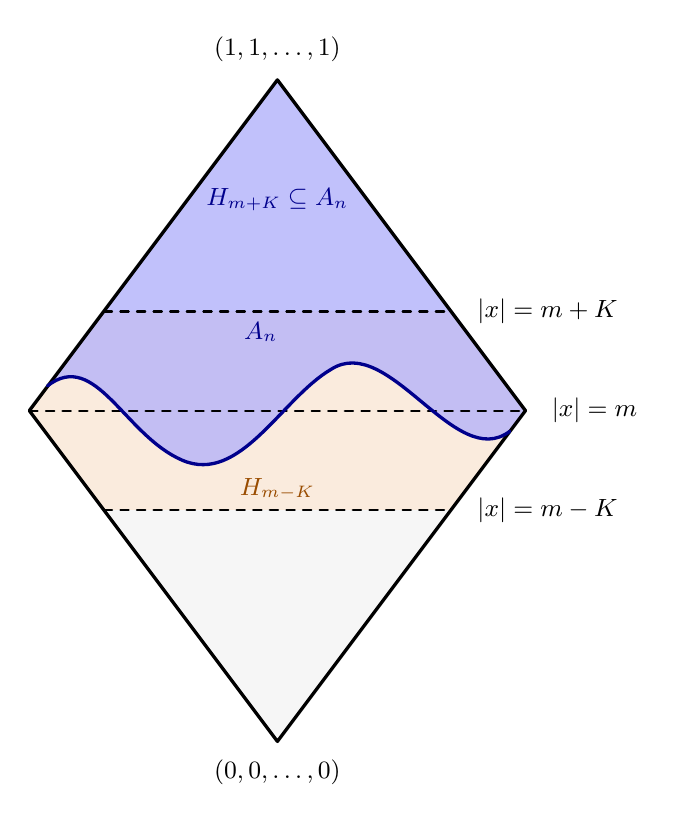
\begin{tikzpicture}[
    scale=1.05,
    line cap=round,
    line join=round,
    >=Latex,
    plane/.style={thick, dashed},
    boundary/.style={very thick, blue!55!black},
    labelstyle/.style={font=\small}
]

% Diamond vertices
\coordinate (Top)    at (0,4);
\coordinate (Bottom) at (0,-4);
\coordinate (Left)   at (-3,0);
\coordinate (Right)  at (3,0);

% Horizontal levels:
% H_{m+K} is above H_m, H_{m-K} is below H_m.
\coordinate (Uleft)  at (-2.1,1.2);
\coordinate (Uright) at (2.1,1.2);

\coordinate (Mleft)  at (-3,0);
\coordinate (Mright) at (3,0);

\coordinate (Lleft)  at (-2.1,-1.2);
\coordinate (Lright) at (2.1,-1.2);

% Boundary of the random monotone set A.
% This boundary lies between H_{m+K} and H_{m-K}.
\coordinate (Gleft)  at (-2.78,0.30);
\coordinate (Gright) at (2.81,-0.25);

% Draw the ambient hypercube as a diamond
\path[fill=gray!7] (Top) -- (Right) -- (Bottom) -- (Left) -- cycle;

% The slab between H_{m+K} and H_{m-K}
\path[fill=orange!25, opacity=0.45]
    (Uleft) -- (Uright) -- (Right) -- (Lright) --
    (Lleft) -- (Left) -- cycle;

% Shade the monotone set A.
% It contains everything above H_{m+K}, and stops above H_{m-K}.
\path[fill=blue!35, opacity=0.65]
    (Top) -- (Right) -- (Gright)
    .. controls (2.15,-0.75) and (1.35,0.95) .. (0.65,0.50)
    .. controls (0.05,0.15) and (-0.45,-0.90) .. (-1.15,-0.60)
    .. controls (-1.85,-0.30) and (-2.20,0.75) .. (Gleft)
    -- cycle;

% Outline of the diamond
\draw[very thick] (Top) -- (Right) -- (Bottom) -- (Left) -- cycle;

% Draw the three threshold planes
\draw[plane] (Uleft) -- (Uright);
\draw[plane] (Mleft) -- (Mright);
\draw[plane] (Lleft) -- (Lright);

% Draw the fluctuating boundary of A
\draw[boundary]
    (Gright)
    .. controls (2.15,-0.75) and (1.35,0.95) .. (0.65,0.50)
    .. controls (0.05,0.15) and (-0.45,-0.90) .. (-1.15,-0.60)
    .. controls (-1.85,-0.30) and (-2.20,0.75) .. (Gleft);

% Labels for vertices
\node[labelstyle, above=3pt] at (Top) {$(1,1,\ldots,1)$};
\node[labelstyle, below=3pt] at (Bottom) {$(0,0,\ldots,0)$};

% Labels for planes
\node[labelstyle, right=6pt] at (Uright) {$|x|=m+K$};
\node[labelstyle, right=6pt] at (Mright) {$|x|=m$};
\node[labelstyle, right=6pt] at (Lright) {$|x|=m-K$};

% Region labels
\node[labelstyle, blue!55!black] at (0,2.55) {$H_{m+K}\subseteq A_n$};
\node[labelstyle, blue!55!black] at (-0.2,0.95) {$A_n$};
\node[labelstyle, orange!60!black] at (0,-0.95) {$H_{m-K}$};

% Optional annotation for the random boundary
%\node[labelstyle, blue!55!black, align=center] at (0.2,-1.75)
%    {random monotone\\boundary of $A$};

%\draw[->, blue!55!black]
  %  (0.05,-1.35) to[bend left=20] (-0.65,-0.55);

\end{tikzpicture}
\caption{Illustration of a random monotone subset $A_n\subseteq \Omega_n$}
\label{fig:RandomMonotoneSet}
\end{figure}





\section{Log-Sobolev inequality for Hamming caps}\label{sec:LSI-caps}

The goal of this section is to prove the following estimate. 

\begin{theorem}[Sharp LSI for Hamming caps]\label{thm:hamming-caps}
For every $0\leq s< n$, 
\[
 t_{\operatorname{LS}}(H_s)  \asymp
        n\log\frac{en}{n-s+1}.
\]
\end{theorem}

We write $\pi_s$ for the uniform measure on $H_s$, and $\Ecal_s$ for the Dirichlet form of the censored walk on $H_s$. Let $p_k=\pi_s(E_k)$ and $\nu_k$ be the uniform measure on $E_k$. 

Throughout the section, we denote $X_k\sim \nu_k$, and we write $X_k^{\uparrow}$ (resp. $X_k^{\downarrow}$) for the random point obtained from $X_k$ by flipping a uniformly chosen zero-coordinate (resp. one-coordinate) to one (resp. zero). More precisely, conditionally on $X_k=x$, we have 
$$
\mathbb{P}(X_k^\uparrow=y\mid X_k=x)
=\frac{1}{n-k}\mathbf 1_{\{y\in E_{k+1},\, y\sim x\}}.
$$
Notice also that $X_k^{\uparrow}\sim\nu_{k+1}$ and that $(X_k,X_k^{\uparrow})$ has the same law as $(X_{k+1}^{\downarrow}, X_{k+1})$. By reversibility, every edge of the censored walk inside $H_s$ may be counted once, oriented from $E_k$ to $E_{k+1}$. Hence
\begin{align}
\Ecal_{H_s}(f,f)&= \frac{1}{2n|H_s|}
\sum_{k=s}^{n-1} \sum_{\substack{x\in E_k,\, y\in E_{k+1}\\ x\sim y}} (f(y)-f(x))^2  \nonumber \\
&=\sum_{k=s}^{n-1} p_k\frac{n-k}{2n}
\mathbb{E}{
\bigl(f(X_k^\uparrow)-f(X_k)\bigr)^2}\label{eq:Dir-up-walk},
\end{align}
%where the expectation in  the $k$-th term is over $(X_k,X_k^{\uparrow})$. 

Our starting point is the entropy decomposition with respect to the partition $H_s=\cup_{k\geq s}E_{k}$, which separates a radial contribution corresponding to the distribution across the Hamming levels, from a tangential contribution corresponding to the oscillation within each level.  

\begin{lemma}[Entropy decomposition]\label{lem:entropy-decomp}
For every $0\le s \le n$ and $f:\, H_s\to \R$, we have
$$     
\Ent_{\pi_s}(f^2) =\Ent_{p}(\bar{f}^2)+\sum_{k= s}^{n-1}p_{k}\Ent_{\nu_k}(f^2),
$$
where $\bar{f}:\, \{s,\ldots,n\}\to \R$ is defined by $\bar{f}(k)= (\mathbb{E}_{\nu_k}f^2)^{\frac12}=\Vert f(X_k)\Vert_{L^2}$. 
\end{lemma}


The radial contribution corresponds to a log-Sobolev inequality for a birth-death chain, which is well studied and follows, for instance, from the Hardy-type criteria for birth-death chains (see~\cite{Miclo}). In the present setting, however, the needed bound follows immediately from the log-Sobolev inequality on the full cube. We include the short argument for completeness.

\begin{proposition}[Radial contribution]
\label{prop:radial-contribution}
For every $0\leq s\le n-1$ and $f:\, H_s\to \R$, 
$$
\Ent_{p}(\bar{f}^2)\leq  2\,n\, \Ecal_{H_s}(f,f).
$$
\end{proposition}
\begin{proof}
Given $0\leq s\le n-1$ and $u:\, \{s,\ldots, n\}\to \R$, we define its radial extension $U:\, \{0,1\}^n\to \R$ by $U(x)= u(s\vee |x|)$. Note that $U$ is constant on $H_s^c$ and $U(x)=u(|x|)$ on $H_s$. Let $X\sim \pi_s$. Since the law of $|X|$ under $\pi_s$ is $p=(p_s,\ldots,p_n)$, we have 
$$
\Ent_{\pi_s}(U^2\vert_{H_s})= \Ent_{p}(u^2)
$$
This, together with the entropy decomposition with respect to the partition $\Omega_n=H_s\cup H_s^c$, implies that  
$$
\Ent_{\pi}(U^2)\geq \pi(H_s)\Ent_{\pi_s}(U^2\vert_{H_s})= \pi(H_s) \Ent_{p}(u^2).
$$
Using the log-Sobolev inequality $\Ent_{\pi}(U^2)\leq 2n\Ecal_{\Omega_n}(U, U)$ for the full cube~\cite[Theorem 5.1]{BLM} and observing that 
$$
\Ecal_{\Omega_n}(U,U)= \pi(H_s) \sum_{k=s}^{n-1} p_k \frac{n-k}{2n} \big(u(k+1)-u(k)\big)^2,
$$
we deduce 
$$
\Ent_{p}(u^2)\leq 2\,n\,\sum_{k=s}^{n-1} p_k \frac{n-k}{2n} \big(u(k+1)-u(k)\big)^2. 
$$
Applying this to $u=\bar{f}$, and using the triangle inequality 
$$
|\bar{f}(k+1)-\bar{f}(k)|\leq  \Vert f(X_k^{\uparrow})-f(X_k)\Vert_{L^2},
$$
the result follows in view of \eqref{eq:Dir-up-walk}.

\end{proof}
We now turn to the entropy inside the Hamming levels. The natural auxiliary chain on $E_k$ is the Bernoulli-Laplace chain \cite[Section XV.2]{Feller1}: from $x\in E_k$, pick two coordinates $i$ and $j$ at random and swap their values, that is, we define a new $x^{(ij)}\in \Omega_n$ by swapping the $i$-th and the $j$-th coordinates of $x$ and keeping the rest of the coordinates unchanged. 

Following~\cite{LeeYau}, we define the Dirichlet energy of the Bernoulli-Laplace chain on $E_k$ as
\begin{align*}
    \Ecal^{\operatorname{BL}}_{k}(g,g):=\frac{1}{2n}\mathbb{E}\left[\sum_{i,j: i<j}\left(g(X_k)-g(X^{(ij)}_k)\right)^2\right]
\end{align*}
We rewrite the Dirichlet energy in a more convenient form. Given $X_k=x\in E_{k}$, let $(u, v)$ be such that $u$ is a uniformly random zero coordinate in $x$ and $v$ is a uniformly random one coordinate in $x$. Then, 
\begin{align}
\label{eqn:BL-Dir}
    \Ecal^{\operatorname{BL}}_{k}(g,g):=\frac{k(n-k)}{2n}\mathbb{E}\left[\left(g(X_k)-g(X^{(uv)}_k)\right)^2\right]\;,
\end{align}
where the expectation is with respect to the tuple $(X_k,u,v)$ where $X_k\sim \nu_k$. 


\begin{lemma}[Up-down representation of Bernoulli-Laplace]\label{lem:up-down-BL}
   Let $1\leq k\leq n-1$. Then, for every $g:\, \Omega_n\to \R$, we have 
   $$
   \Ecal^{\operatorname{BL}}_k(g,g)\leq \frac{(k+1)(n-k)}{n} \mathbb{E}\left[(g(X^{\uparrow}_k)-g(X_k))^2\right], 
   $$
   and 
    $$
   \Ecal^{\operatorname{BL}}_k(g,g)\leq \frac{k(n-k+1)}{n} \mathbb{E}\left[(g(X^{\downarrow}_k)-g(X_k))^2\right]. 
   $$
\end{lemma}
% \begin{proof}
%     We prove the upward estimate, since the downward one is identical upon exchanging zeros and ones. Note that the summation in $\Ecal^{\operatorname{BL}}_k$ is over $i<j$ such that $X_i+X_j=1$. In this case, there exists a unique $Z_{k+1}=X_k \vee X_k^{(ij)}\in E_{k+1}$. Condition on $Z_{k+1}$, $X_k$ and $X_k^{(ij)}$ are independent, and both follow the law of $Z_{k+1}^\downarrow$. Therefore,
%     \begin{align*}
%         \Ecal^{\operatorname{BL}}_k(g,g)=\frac{1}{2n}\E{\E{\sum_{i<j}\left(g(X_k)-g(X_k^{(ij)})\right)^2\Big| Z_{k+1}}}
%     \end{align*}
%     As there are $2k(n-k)$ such pairs $i<j$, we get that
%     \begin{align*}
%         \Ecal^{\operatorname{BL}}_k(g,g)=\frac{k(n-k)}{n}\E{\E{\left(g(Z)-g(Z')\right)^2\Big| Z_{k+1}}},
%     \end{align*}
%     where $Z,Z'$ are independent copies of $Z_{k+1}^\downarrow$, given $Z_{k+1}$. Therefore,
%     \begin{align*}
%         \Ecal^{\operatorname{BL}}_k(g,g)=\frac{k(n-k)}{n}\E{\operatorname{var}\left(g(Z_{k+1}^\downarrow)\right)\Big|Z_{k+1}}\le \frac{k(n-k)}{n}\E{\left(g(Z_{k+1}^\downarrow)-g(Z_{k+1})\right)^2}
%     \end{align*}
%     It suffices to note that the distribution of $(Z_{k+1}^\downarrow,Z_{k+1})$ is equal to the distribution of $(X_k,X_k^\uparrow)$.



% Note that 
% $$
% \Ecal_{K_kK_k^*}(g,g)= \langle g, (I-K_kK_k^*)g\rangle_{\nu_k}= \E{g(X_k)^2}-\E{(K_k^*g)(X_k^{\uparrow})^2}, 
% $$
% and since $(K_k^*g)(X_k^{\uparrow})= \E{g(X_k)\mid X_k^{\uparrow}}$, we obtain 
% $$
% \Ecal_{K_kK_k^*}(g,g)= \E{\var(g(X_k)\mid X_k^{\uparrow})}\leq \E{(g(X_k)-g(X_k^{\uparrow}))^2}.
% $$
% Putting the above together finishes the proof. 
% \end{proof}


\begin{proof}
We prove the upward estimate, since the downward one is identical upon exchanging zeros and ones. 
%Let $X\sim \nu_k$. 
% We start by writing $\Ecal_{k}^{BL}(\cdot, \cdot)$ in a more convenient form. To this end, let $I, J$ be independent and uniform on $\{1, \ldots, n\}$. Then, 
% \[
% \Ecal_k^{BL}(g, g) = \frac{n}{4}\mathbb{E}_{\nu_k}\mathbb{E}_{I, J}(g(X)-g(X^{(IJ)}))^2\;.
% \]
% Note that conditional on $X$, the probability that $X({I})=0$ and $J=I$ or $X_{J}=1$ is $(n-k)(k+1)/n^2$. On the complement of this event, we have $X=X^{(IJ)}$. Therefore, 
% \[
% \Ecal_k^{BL}(g, g)  = \frac{(n-k)(k+1)}{4n}
% \]
Given $X_k=x\in E_k$, let $I$ be a uniform random zero coordinate in $x$ and let $X^{\uparrow}_k=X_k+e_{I}\in E_{k+1}$. Let $J$ be a uniform random one coordinate in $X_k^\uparrow$ (independent of $I$), and let $Z_k=(X_k^\uparrow)^{\downarrow}=X_k^\uparrow-e_J$. Note that $X_k\ne Z_k$ with probability $k/(k+1)$. Furthermore, given $X_k\neq Z_k$, $(I, J)$ has the same distribution as $(u, v)$. In particular, 
\[
\mathbb{E}\left[\left(g(X_k)-g(Z_k)\right)^2\right] = \frac{k}{k+1}\mathbb{E}\left[\left(g(X_k)-g(X^{(uv)}_k)\right)^2\right]\;.
\]
Combining with~\eqref{eqn:BL-Dir}, we get
\[
    \mathcal{E}_k^{BL}(g, g) = \frac{(n-k)(k+1)}{2n} \mathbb{E}\left[\left(g(X_k)-g(Z_k)\right)^2\right]\;.
\]
We now observe that $X_k$ and $Z_k$ are independent given $X^\uparrow_k$, as $I$ and $J$ are independent. Furthermore, given $X_k^\uparrow$, $X_k$ and $Z_k$ have the same distribution as the distribution of $(X^\uparrow_k)^\downarrow$. Therefore,
    \[
    \frac{1}{2}\mathbb{E}\left[\left(g(X_k)-g(Z_k)\right)^2\vert X^\uparrow_k \right]=\var(g(X_k)\vert X_k^\uparrow)\leq \mathbb{E}\left[\left(g(X_k)-g(X_k^\uparrow)\right)^2\Big| X_k^\uparrow\right]\;.
    \]
The result follows by taking the expectation.
\end{proof}


\begin{proposition}[Tangential contribution]\label{prop:tangential-contribution}
    For every $1\leq s\leq n-1$ and $f:\, H_s\to \R$,
    $$
    \sum_{k= s}^{n-1} p_k\Ent_{\nu_k}(f^2)\leq 36\,n \log \frac{en}{n-s}\, \Ecal_{H_s}(f,f). 
    $$
\end{proposition}
\begin{proof}
For every $1\leq k\leq n-1$, we make use of the sharp log-Sobolev inequality for Bernoulli-Laplace (see \cite[Theorem~5]{LeeYau})
%, which, with our normalization, translates to 
    $$
    \Ent_{\nu_k}(f^2)\leq \frac{2}{\log 2} \,\log \frac{n^2}{k(n-k)} \Ecal_{k}^{BL}(f,f).
    $$
   Combined with Lemma~\ref{lem:up-down-BL}, this implies   
   \begin{equation}\label{eq:entropy-upwalk}
       \Ent_{\nu_k}(f^2)\leq \frac{2}{\log 2} \, \frac{(k+1)(n-k)}{n}\log \frac{n^2}{k(n-k)} \mathbb{E}{(f(X^{\uparrow}_k)-f(X_k))^2}\;,
   \end{equation}
    and 
      \begin{equation}\label{eq:entropy-downwalk}
    \Ent_{\nu_k}(f^2)\leq \frac{2}{\log 2} \, \frac{k(n-k+1)}{n}\log \frac{n^2}{k(n-k)} \mathbb{E}{(f(X^{\downarrow}_k)-f(X_k))^2}.
   \end{equation}
Denote, for brevity, 
\begin{align*}
    \Gamma_k=p_k\frac{n-k}{n}\mathbb{E}{\bigl(f(X^\uparrow_k)-f(X_k)\bigr)^2}.
\end{align*}
Using that $p_k=\frac{n-k+1}{k} p_{k-1}$ and $(X_k^{\downarrow}, X_k)\sim (X_{k-1},X_{k-1}^{\uparrow})$, the inequalities \eqref{eq:entropy-upwalk} and \eqref{eq:entropy-downwalk} reduce to 
$$
p_k\Ent_{\nu_k}(f^2)\leq \frac{2}{\log 2} \log \frac{n^2}{k(n-k)} \, \min\big((k+1)\Gamma_{k}, (n-k+1)\Gamma_{k-1}\big).
$$
Using the elementary relation $\min (k+1, n-k+1)\, \log \frac{n^2}{k(n-k)}\leq 2n$, we get that 
$$
\begin{cases}
    p_k\Ent_{\nu_k}(f^2)\leq \frac{4n}{\log 2} \Gamma_{k}  & \text{ if } k\leq n-k;\\
    & \\
     p_k\Ent_{\nu_k}(f^2)\leq \frac{4n}{\log 2} \Gamma_{k-1}  & \text{ otherwise.}
\end{cases}
$$
Summing over $k> s$ and using \eqref{eq:Dir-up-walk}, we get 
$$
\sum_{k=s+1}^{n-1} p_k\Ent_{\nu_k}(f^2)\leq \frac{16\,n}{\log 2}\, \Ecal_{H_s}(f,f).
$$
Finally, we use \eqref{eq:entropy-upwalk} with $k=s$ to get
$$
p_s\Ent_{\nu_s}(f^2)\leq \frac{2(s+1)}{\log 2} \log \frac{n^2}{s(n-s)} \, \Ecal_{H_s}(f,f)\leq \frac{8\,n}{\log 2} \log \frac{en}{n-s}\, \Ecal_{H_s}(f,f). 
$$
Combining the above and using that $\frac{24}{\log 2}\leq 36$, we finish the proof. 
\end{proof}

\begin{proof}[Proof of Theorem~\ref{thm:hamming-caps}]
The case $s=0$ corresponds to the full cube. Therefore, we assume $1\leq s\leq n-1$. The upper bound readily follows by combining Lemma~\ref{lem:entropy-decomp} with Propositions~\ref{prop:radial-contribution} and \ref{prop:tangential-contribution}. 


To get the lower bound, fix $z\in E_s$ and take $f=\mathbf 1_{\{z\}}$. Then, we have 
$$
\Ent_{\pi_s}(f^2)=\frac{\log |H_s|}{|H_s|}. 
$$
On the other hand, $z$ has exactly $n-s$ neighbors inside $H_s$. Therefore, 
$$
\Ecal_{H_s}(f,f)= \frac{n-s}{2n |H_s|}. 
$$
Combining the two identities, we get 
$$
\frac{\Ent_{\pi_s}(f^2)}{\Ecal_{H_s}(f,f)}= \frac{2n\log |H_s|}{n-s}.
$$
It remains to use that $|H_s|\geq \binom{n}{s}$ if $s\geq n/2$ and that $|H_s|\geq 2^{n-1}$ when $s<n/2$. 
\end{proof}



\section{The log-Sobolev inequality for sandwiched monotone sets}\label{sec:LSI-sandwich}

The goal of this section is to transfer the logarithmic Sobolev inequality from Hamming caps to monotone sets lying between two nearby caps. The main ingredient is a one-layer extension lemma: whenever a Hamming layer is added, functions can be extended harmonically to the new vertices while increasing the Dirichlet energy by at most a constant factor. Iterating this extension across the layers of the sandwich yields a comparison theorem between the logarithmic Sobolev constants of the monotone set and the surrounding cap.

\begin{lemma}[One layer harmonic extension]\label{lem:one-step-extension}
    Let $A\subseteq \Omega_n$ be a monotone subset, and for every $0\leq l\leq n-1$, set $D_l=A\cup H_l$. For every $0\leq l\leq n-1$ and every function $f:\, D_{l+1}\to \R$, there exists an extension $F:\, D_{l}\to \R$ such that $F_{\mid D_{l+1}}=f$ and 
    $$
    \Ecal_{D_l}(F,F)\leq \frac{|D_{l+1}|}{|D_l|} \Big(1+\frac{l+2}{n-l}\Big)\, \Ecal_{D_{l+1}}(f,f). 
    $$
\end{lemma}
\begin{proof}
 Fix $0\leq l\leq n-1$, and note that $D_l\setminus D_{l+1}=E_l\setminus A$. For $x\in E_l\setminus A$, let 
 $$
 U(x)=\{y\in E_{l+1}:\, y\sim x\}
 $$
 be the set of upper neighbors of $x$. Since $H_{l+1}\subseteq D_{l+1}$, all these neighbors belong to $D_{l+1}$. 
 Let $f:\, D_{l+1}\to \R$ and define 
 $$
 F(x)=\frac{1}{n-l}\sum_{y\in U(x)} f(y),\quad x\in E_l\setminus A,
 $$
 and set $F=f$ on $D_{l+1}$. 

Let $x\in E_l\setminus A$. We claim that every neighbor of $x$ in $D_{l+1}$ belongs to $U(x)$. Indeed, let $y\in E_{l-1}$ be a neighbor of $x$. Then $y\not\in H_{l+1}$, and if $y\in A$, monotonicity of $A$ would imply that $x\in A$, a contradiction. Therefore $y\not\in D_{l+1}$. 

Thus, the only new edges created when passing from $D_{l+1}$ to $D_l$ are the edges joining $x\in E_l\setminus A$ to its upper neighbors in $U(x)$. Therefore 
\begin{equation}
\label{eq:decomp-Dirichlet}
    \Ecal_{D_{l}}(F, F) = \frac{|D_{l+1}|}{|D_{l}|}\Ecal_{D_{l+1}}(f, f) + \frac{1}{2n|D_{l}|}\sum_{x\in E_l\setminus A}\sum_{y\in U(x)}(F(x)-f(y))^2\;.
\end{equation}
Since $F(x)$ is the average of $f$ on $U(x)$, the variance identity yields 
$$
    \sum_{y\in U(x)}(F(x)-f(y))^2= \frac{1}{2(n-l)} \sum_{y,z\in U(x)} (f(y)-f(z))^2. 
$$
Summing over $x$, and using that every pair $y,z\in E_{l+1}$ with $|y-z|=2$ has at most one common lower neighbor in $E_l$, we get 
\begin{equation}\label{eq:after-variance-identity}
  \sum_{x\in E_l\setminus A}\sum_{y\in U(x)}(F(x)-f(y))^2\leq \frac{1}{2(n-l)} \sum_{\substack{y,z\in E_{l+1}\\ |y-z|=2}}  (f(y)-f(z))^2.
\end{equation}
For such a pair $y,z$, let $w=y\vee z\in E_{l+2}$. Then $w\in H_{l+1}\subseteq D_{l+1}$, and $w$ is adjacent to both $y$ and $z$. Let $L(w)=\{y\in E_{\ell+1}: y\sim w\}$. Write $\bar{f}_{L(w)}=\frac{1}{|L(w)|}\sum_{y\in L(w)}f(y)$ for the average of $f$ over $L(w)$. Using the variance identity over the set $L(w)$, we get 
\[
\frac{1}{2}\sum_{y, z\in L(w)}(f(y)-f(z))^2 = |L(w)|\sum_{y\in L(w)}(f(y)-\bar{f}_{L(w)})^2\leq |L(w)|\sum_{y\in L(w)}(f(y)-f(w))^2\;.
\]
% Hence, 
% $$
% (f(y)-f(z))^2\leq 2(f(y)-f(w))^2+2(f(w)-f(z))^2
% $$
% Now observe that given two neighbors $(y, w)\in E_{l+1}\times E_{l+2}$, there are at most $(l+1)$ choices for $z\in E_{l+1}$ such that $w=y\vee z$. 
Using this together with \eqref{eq:after-variance-identity} and the fact that $|L(w)|=l+2$, we get 
$$
\sum_{x\in E_l\setminus A}\sum_{y\in U(x)}(F(x)-f(y))^2\leq \frac{(l+2)}{(n-l)} \sum_{\substack{y,w\in D_{l+1}\\ y\sim w}}  (f(y)-f(w))^2.
$$
Plugging this back in \eqref{eq:decomp-Dirichlet}, we finish the proof. 
\end{proof}



\begin{theorem}[Comparison for sandwiched monotone sets]\label{thm:sandwich-monotone-set}
    Let $0\leq s\leq r\leq n-1$, and let $A\subseteq \Omega_n$ be a monotone set satisfying 
    $$
    H_r\subseteq A\subseteq H_s. 
    $$
Then 
$$
 t_{\operatorname{LS}}(A)\leq t_{\operatorname{LS}}(H_s)\, \prod_{l=s}^{r-1} \left(1+\frac{l+2}{n-l}\right).
$$
\end{theorem}
\begin{proof}
    For every $s\leq l\leq r$, set $D_l=A\cup H_l$. Observe that $D_s=H_s$ while $D_r=A$. Let $f:\, A\to \R$. Applying Lemma~\ref{lem:one-step-extension} successively for $l=s,\ldots, r-1$ , we obtain an extension $F:\, H_s\to \R$ of $f$ satisfying 
    \begin{equation}\label{eq:dirichlet-comparison}
        \Ecal_s(F,F)\leq \frac{|A|}{|H_s|}\prod_{l=s}^{r-1} \left(1+\frac{l+2}{n-l}\right)\, \Ecal_A(f,f). 
    \end{equation}
We now compare the entropies. Since $F_{\mid A}=f$, the entropy decomposition associated with the partition $H_s=A\cup (H_s\setminus A)$ gives 
\begin{equation}\label{eq:entropy-comparison}
   \Ent_{\pi_s}(F^2)\geq \frac{|A|}{|H_s|} \Ent_{\pi_A}(f^2). 
\end{equation}
Applying the log-Sobolev inequality on $H_s$, and combining it with \eqref{eq:dirichlet-comparison} and \eqref{eq:entropy-comparison}, we get
$$
\Ent_{\pi_A}(f^2)\leq t_{\operatorname{LS}}(H_s)  \prod_{l=s}^{r-1} \left(1+\frac{l+2}{n-l}\right)\, \Ecal_A(f,f).
$$
The statement follows. 
\end{proof}


\begin{proof}[Proof of Theorem~\ref{thm:highprobLSI}]
    Let $A_n$ be a uniformly chosen monotone subset of $\Omega_n$. By \eqref{eqn:TypicalA}, there exists a universal constant $K$ such that 
$$
    \mathbb{P}(H_{m+K}^{(n)}\subseteq A_n\subseteq H_{m-K}^{(n)})=1-o_n(1)\;.
$$
On this event, Theorem~\ref{thm:sandwich-monotone-set} together with Theorem~\ref{thm:hamming-caps} yields
$$
 t_{\operatorname{LS}}(A_n)\leq C_K  t_{\operatorname{LS}}(H_{m-K})\leq C_K' n,
$$
for some constants $C_K, C_K'$ depending only on $K$. 
To prove the matching lower bound, note that on the same event we have $H_{m+K}\subseteq A_n$ and therefore 
$$
\operatorname{diam}(A)\ge \operatorname{diam}(H_{m+K})\ge \frac{n}{2}-K.
$$
It remains to use a diameter lower bound for the logarithmic Sobolev constant (see \cite[Lemma 1]{SY25}) to conclude the proof. 
\end{proof}


\section{Monotone sets with large log-Sobolev constant}\label{sec:large-LSI}

In this section, we investigate monotone sets with large log-Sobolev constants. We show that the largest possible order is $n^2$ and that this order is attained by monotone sets that occupy at least a constant fraction of the hypercube. The lower bound arises from a simple bottleneck mechanism. Let $A\subseteq \Omega_n$ and $U\subseteq A$, and define the \emph{edge boundary} as 
\[
\partial_{A}U :=\{\{x, y\}: x\in U, y\in A\setminus U, x\sim y\}\;.
\] 
Applying the logarithmic Sobolev inequality to the indicator function $\mathbf{1}_U$ yields 
\begin{align}\label{equation: universal lower bound}
    t_{\operatorname{LS}}(A)\geq 2n\cdot \frac{|U|\,\log (|A|/|U|)}{|\partial_AU|}\;.
\end{align}
The lower bound depends not only on the size of the boundary $\partial_AU$, but also on the relative size of $U$ inside $A$. Consequently, a subset $U$ may force a large logarithmic Sobolev constant even when its boundary is comparable to its volume, provided that $U$ occupies only an exponentially small fraction of $A$. We end this section with a simple example to illustrate this. 

\begin{proposition}[Worst-case behavior at fixed density]\label{prop:wortcase-LSI}
    Let $\alpha\in (0,1/2]$ be fixed. Then 
    $$
     \sup_{\substack{A\subseteq \Omega_n \text{ monotone}\\ |A|\geq \alpha |\Omega_n|} }t_{\operatorname{LS}}(A)  \asymp_\alpha n^2
    $$
\end{proposition}

\begin{proof}
We begin with the upper bound. Let $A\subseteq \Omega_n$ be a monotone set $|A|\geq \alpha|\Omega_n|$. By the log-Sobolev inequality for the rank-one chain \cite[Theorem 2.2.9]{S-C97}, there exists a universal constant $C$ such that
   $$
   \Ent_{\pi_A}(f^2)\leq C\log  |A|\, \var_{\pi_A}(f),
   $$
   for any function $f:\, A\to \R$.
   
On the other hand, the sharp Poincaré inequality for monotone sets \cite{fei2025spectral} yields 
$$
\var_{\pi_A}(f)\leq C' n \Ecal_A(f,f),
$$
for some constant $C'$ depending only on $\alpha$. Combining the two estimates and using the fact that $|A|\leq |\Omega_n|=2^n$ yields the upper bound. 

For the reverse inequality, fix $q=q(\alpha)\geq 1$ satisfying $1-2^{-q}\geq \alpha$. Write $n=m+q$ and define 
$$
A_{n,q}= \{(u,v)\in \{0,1\}^{m}\times \{0,1\}^q:\, v\neq 0\}\cup \{z\},
$$
where $z$ is the vector whose first $m$ coordinates are equal to one and its last $q$ are equal to zero. 
Clearly, $A_{n,q}$ is a monotone set and 
$|A_{n,q}|= (1-2^{-q})2^n+1\geq \alpha |\Omega_n|$.
Note that $z$ has exactly $q$ neighbors in $A_{n,q}$. Therefore, setting $U=\{z\}$ in \eqref{equation: universal lower bound} , we get
\begin{align*}
    t_{\operatorname{LS}}(A_{n,q})\geq \frac{2n \log |A_{n,q}|}{q}.
\end{align*}
The proof is complete once the lower bound on $|A_{n,q}|$ is used.
%Consequently, setting $f=\mathbf{1}_{\{z\}}$, we have 
%$$
%\Ent_{\pi_{A_n,q}}(f^2)=\frac{1}{|A_{n,q}|}\log |A_{n,q}|,
%$$
%while 
%$$
%\Ecal_{A_{n,q}}(f,f)= \frac{q}{2n|A_{n,q}|}.
%$$
%Hence, 
%$$
%t_{\operatorname{LS}}(A_{n,q})\geq \frac{2n \log |A_{n,q}|}{q},
%$$
%and the proof is complete once the lower bound on $|A_{n,q}|$ is used.
\end{proof}


\iffalse
\begin{remark}[Mixing time in the example]
We provide the sketch of an argument to show that the mixing time is $O(n\log n)$. Peres and Sousi~\cite{PS15} showed that the mixing time of a lazy, reversible Markov chain is comparable to the hitting time of large sets. More precisely, for any $\gamma\in (0, 1/2)$, there are constant $c_{\gamma}, C_{\gamma}$ such that 
\[c_{\gamma}t_{H}(\gamma)\leq t_{\mix}\leq C_{\gamma}t_{H}(\gamma),\]
where 
\[t_{H}(\gamma) = \sup_{y\in \Omega}\sup_{B\subseteq\Omega: \mu(B)\geq \gamma} \mathbb{E}_{y}[\tau_{B}]\;.\]

Let $A\equiv A_{n, q}$ be as above and $A'=A\setminus\{z\}$ and let $(X_t)_{t}$ denote the censored chain on $A$. Then, 
\[
t_{\mix}(A)\leq C_{\gamma}t_{H}^{X}(\gamma)\;,
\]
Replacing $B\subseteq A$ by $B\cap A'$ (and replacing $\gamma$ by $\gamma/2$), we can assume that $B\subseteq A'$. Furthermore, if the walk starts at $z$, we note that 
\[
\mathbb{E}_z[\tau_{B}]\leq \mathbb{E}_z[\tau_{A'}]+\sup_{y\in A'}\mathbb{E}_{y}[\tau_{B}]\;.
\]
Since $\mathbb{E}_z[\tau_{A'}]=O_{q}(n)$, it suffices to show that 
\[
\sup_{y\in A'}\sup_{B\subseteq A': \pi(B)\geq \gamma} \mathbb{E}_{y}^{X}[\tau_{B}] = O_{\gamma, q}(n\log n)\;.
\]
Now, let $Y=(Y_t)_t$ denote the censored chain on $A'$. This is a lazy random walk on $m$-dimensional cube--slowed by a factor of $n/m$. The usual mixing time bound for the lazy random walk on cubes, combined with Peres-Sousi, gives us that 
\[
\sup_{y\in A'}\sup_{B\subseteq A': \pi(B)\geq \gamma} \mathbb{E}_{y}^{Y}[\tau_{B}] =O_{\gamma, q}(n\log n)\;.
\]

Now fix $y\in A'$ and $B\subseteq A'$ such that $\pi(A)\geq \gamma$. We want to couple the walks $X$ and $Y$ starting at $y$ so that 


\end{remark}

\fi





% \begin{remark}
% On discrete state spaces, another important functional inequality is the modified log-Sobolev inequality (MLSI) that measures the entropy-production along the semigroup~\cite{bobkov2006modified}. The modified log-Sobolev constant $t_{\operatorname{MLS}}(P)$ for a Markov chain $P$ with stationary measure $\pi$ on a finite state space $\Omega$ is defined as the smallest constant such that 
% \begin{equation}
% \label{eqn:MLSIDef}
%     \Ent_{\pi}(f)\leq t_{\operatorname{MLS}}(P)\,\Ecal_{P}(f, \log f),
% \end{equation}
% for every $f:\Omega\to (0, \infty)$. For a monotone set $A\subseteq \Omega_n$, we use $t_{\operatorname{MLS}}(A)$ to denote the modified log-Sobolev constant for the random walk censored to $A$. Using the classical inequality that $t_{\operatorname{MLS}}(P)\leq t_{\operatorname{LS}}(P)/4$ and~\cite[Theorem 1]{STY23}, we conclude that 
% $$
%    \frac{c_{\alpha}n^2}{\log n} \leq \sup_{\substack{A\subseteq \Omega_n \text{ monotone}\\ |A|\geq \alpha 2^n} }t_{\operatorname{MLS}}(A) \leq C_{\alpha} n^2,
% $$
% for some constant $c_{\alpha}, C_{\alpha}>0$. 


% On the other hand, the proof of Theorem~\ref{thm:hamming-caps} can be readily adapted to show that $t_{\operatorname{MLS}}(H_s)\asymp n$ for all $1\leq s<n$. We sketch the proof briefly and leave the details to the reader. Set $\Phi(a, b) = (a-b)(\log a-\log b)$ and notice that
%     \[
%     \Ecal_{H_s}(f, \log f) = \sum_{k=s}^{n-1}p_k\frac{n-k}{n}\mathbb{E}\left[\Phi(f(X_k), f(X_k^{\uparrow}))\right]\;.
%     \]
%     In Proposition~\ref{prop:radial-contribution}, we instead use the MLSI for the full cube~\cite[Example 3.7]{bobkov2006modified} to get
%     \[
%     \Ent_{p}(\overline{f}^2)\leq n\Ecal_s(f, \log f)\;.
%     \]
%     The proof of Lemma~\ref{lem:up-down-BL} readily adapts to show that
%     \[
%     \Ecal_{B_k}(f, \log f) \leq \frac{k+1}{k}\mathbb{E}\left[\Phi(f(X_k), f(X_k^{\uparrow}))\right]\;.
%     \]
% In the proof of Proposition~\ref{prop:tangential-contribution}, we use the MLSI~\cite{GQ03} for the Bernoulli-Laplace chain~\cite[Example 3.1]{Goel04} to get
% \[
% \Ent_{\nu_k}(f^2)\leq C\frac{k(n-k)}{n}\Ecal_{B_k}(f, \log f)\;\;.
% \]
% Since $k\leq n$, we conclude that 
% \[
% \sum_{k=s}^{n-1}p_k\Ent_{\nu_k}(f^2)\leq Cn\sum_{k=s}^{n}p_k\frac{n-k}{n}\Ecal_{\nu_k}{\Phi(f(X_k), f(X_k^{\uparrow}))}=Cn\Ecal_{H_s}(f, \log f)\;.
% \]
% On the other hand, testing against the function $f=\mathbf{1}\{x_1=0\}$ in~\eqref{eqn:MLSIDef}, one obtains that $t_{\operatorname{MLS}}(H_s)\geq \frac{n}{4}$ for all $0\leq s<n$.
% \end{remark}

% The comparison theorem~\ref{thm:sandwich-monotone-set} readily adapts to the Dirichlet energy of the MLSI, and therefore, we conclude the following. 
% \begin{theorem}[MLSI for typical monotone set]
% Let $A_n$ be a uniformly chosen random monotone subset of $\Omega_n$. There exist universal constants $c, C>0$ such that
% \[
%     \mathbb{P}\left(c\cdot n\leq  t_{\operatorname{MLS}}(A_n)\leq C\cdot n\right) = 1-o_n(1).
% \]
% \end{theorem}

\begin{remark}
    Even though the examples in Proposition~\ref{prop:wortcase-LSI} have a logarithmic Sobolev constant of order $n^2$, they do not contradict the conjecture of Ding and Mossel. Indeed, the obstruction comes from the exceptional vertex $z$, whose mass is exponentially small. While the presence of $z$ forces $t_{\operatorname{LS}}(A)  \asymp_\alpha n^2$, the mean time to leave $z$ is of order $n$. After leaving $z$, the walk behaves essentially like a product chain, suggesting the mixing time remains of order $n\log n$. 

    The same example also shows that the modified logarithmic Sobolev inequality \cite{bobkov2006modified} cannot hold with a constant of order $n$; in fact, the above example provides a lower bound of order $n^2/\log n$. On the other hand, the arguments in Section~\ref{sec:LSI-caps} and \ref{sec:LSI-sandwich} extend with minor modifications, yielding order $n$ modified logarithmic Sobolev constant for all Hamming caps $H_s$, $1\leq s\leq n-1$, and for a random monotone set. 
\end{remark}

\section*{Acknowledgment.}
This work is supported in part by the NYUAD Center for Interdisciplinary Data Science \& AI (CIDSAI), funded by Tamkeen under the NYUAD Research Institute Award CG016.

\bibliographystyle{alpha} % can use amsalpha but repeated authors are dashed
\bibliography{ref}
%%%%%%%%%%%%






\end{document}

\section*{Author affiliations}

\noindent Patrick Oliveira Santos: Division of Science, NYU Abu Dhabi, Saadiyat Island, Abu Dhabi, UAE. \texttt{\small e-mail: po2150@nyu.edu}.\\


\noindent Raghavendra Tripathi: Division of Science, NYU Abu Dhabi, Saadiyat Island, Abu Dhabi, UAE. \texttt{\small e-mail: r.tripathi@nyu.edu}.\\

\noindent Pierre Youssef: 
Division of Science, NYU Abu Dhabi, Saadiyat Island, Abu Dhabi, UAE \& Courant
Institute of Mathematical Sciences, New York University, 251 Mercer st, New York,
NY 10012, USA. 
\texttt{\small e-mail:  yp27@nyu.edu}.

 Choose a one-coordinate and a zero-coordinate uniformly and swap their values. Its appearance here is not accidental. 
%Indeed, let $K_k:\, E_k\to E_{k+1}$ denotes the up operator and let $K_k^*:\, E_{k+1}\to E_{k}$ be its adjoint with respect to $\nu_k$ and $\nu_{k+1}$.
%Indeed, let $\mathcal{E}_k=\{g: E_k \to \R\}$ and $U_k:\mathcal{E}_k \to \mathcal{E}_{k+1}$ denotes the up operator defined by 
%\begin{align*}
%    U_k g(x)=\frac{1}{k+1}\sum_{\substack{y\in E_k\\ y\sim x}}g(y),
%\end{align*}
%for any $g\in \mathcal{E}_k$ and $x\in E_{k+1}$.
%Then, the multiplicative reversibilization $K_kK_k^*$ is a lazy Bernoulli-Laplace chain. 
The following lemma records this relation and allows us to compare the Bernoulli-Laplace energy to the vertical energy in the Hamming cap. 

   
   
   Let us define the Dirichlet energy for the non-lazy version of the Bernoulli-Laplace chain. Pick a zero coordinate and a one coordinate uniformly at random and swap them. Let us denote the transition matrix of this chain as $P$. It is easy to see that the transition matrix $Q$ of the lazy Bernoulli-Laplace chain is $Q=\frac{1}{k+1}I+\frac{k}{k+1}P$.

   

   
Note that $X$ has the same law as $Y^{\downarrow}$ given $Y$. Taking expectation over $Y\sim \nu_{k+1}$, we get  
   \[
    \frac{1}{2}\mathbb{E}\left[\left(g(X)-g(Z)\right)^2\right]\leq \mathbb{E}\left[(f(Y)-f(Y^{\downarrow}))^2\right] = \mathbb{E}\left[(f(Y)-f(Y^{\uparrow}))^2\right]\;,
   \]
   where the last equality follows from the fact that if $Y\sim\nu_{k+1}$ and $Y'\sim \nu_{k}$ then $(Y, Y^{\downarrow})$ has the same law as $(Y'^{\uparrow}, Y')$.
   % In particular, we get 
   % \[
   % \mathcal{D}(g, g)\leq \frac{k}{n}\mathbb{E}_{\nu_{k}}(f(Y)-f(Y^{\uparrow}))^2\;,
   % \]
   Putting everything together finishes the proof.
